\section{Der Visualisierungsprozess [FK]}
\section{Einrichten von AWS}
In AWS [\ref{ssec:aws} eingeloggt hat man die Auswahl von 175 Services. Davon wählt man den Punkt EC2 aus. Mit EC2 kann man Visualisierte Rechner benutzen, um alles Mögliche zu hosten. Um eine Maschine für Elasticsearch und Kibana zu beantragen, geht man auf den Button „Launch Instance“. Im Wizard gibt es nun mehrere Möglichkeiten, welches Betriebssystem auf der VM [\ref{sec:VM}] laufen soll. In unserem Fall Ubuntu Server 18.04 LTS (HVM) (64-Bit, x86). Als Nächstes kann man auswählen, welche Hardware der VM zu Verfügung gestellt werden sollen. Für ES (Elasticsearch) und Kibana braucht man mindestens den Typ "t2.medium" was hauptsächlich an dem benötigten Arbeitsspeicher liegt. Zum Schluss muss man eine Security Group im gleichnamigen Tab erstellen. Sofern man direkt von außen auf die ES DB zugreifen möchte, muss man zumindest den Port 9200 öffnen. Wenn man Multi-nodes einrichten will, muss man Port 9300 öffnen damit die Nodes [\ref{sec:Node}] untereinander kommunizieren können. 
Nun ist die Konfiguration der Virtual Machine fertig. Mit Putty oder ssh kann man sich nun auf die VM verbinden. Der Nachteil bei so einer „billigen“ Hardware Konfiguration ist jedoch das sich die IP und der DNS [\ref{sec:DNS}] bei jedem Neustart ändert. Sodass man nicht ein und dieselbe Adresse immer verwenden kann. Das Passwort bleibt jedoch gleich und man kann sich ein Key File generieren lassen.
Ist man einmal verbunden, installiert man sofort Docker und docker-compose.
Docker install: (vgl. \cite{DockerInstall})
Docker-compose install: (vgl. \cite{DockerComposeInstall})
\section{Installierung von Elasticsearch und Kibana}
Kibana kann als Desktop Version direkt von der Homepage, mit diversen Package Managern oder als Docker Container heruntergeladen werden. Es gibt außerdem eine Möglichkeit sich direkt auf die Elastic Cloud zu verbinden. Ich habe zum Aufsetzen des ELK Stack (Elasticsearch + Kibana) ein eigenes docker-compose geschrieben um automatisch die Container für Elasticsearch und Kibana zu erstellen.
\begin{figure}[H]
    \centering
    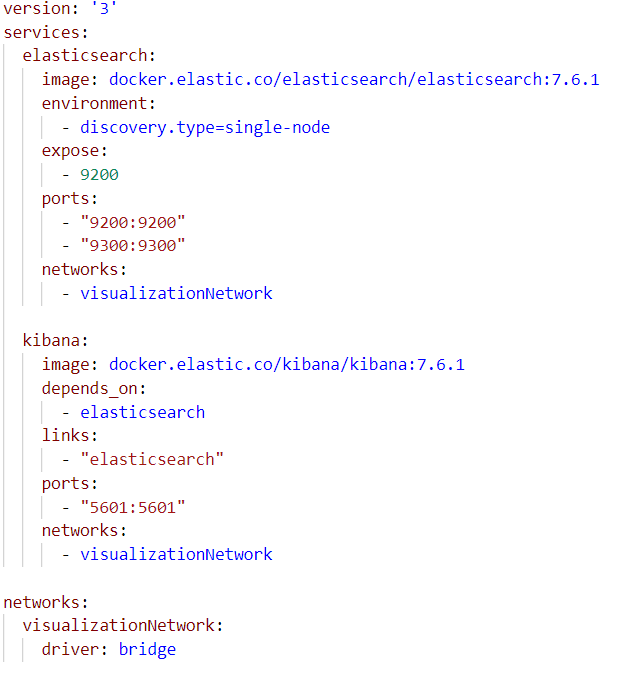
\includegraphics{images/docker-compose_kibana.PNG}
    \caption{docker-compose zum Aufsetzen von ES und Kibana}
    \label{iziellen Elastic Homepage runtergeladen falls sie noch nicht lokalmg:docker-compose_kibana}
\end{figure}
Beide Images werden von der offiziellen Elastic Homepage runtergeladen, falls sie noch nicht lokal, existieren.
Da es bei dem Prototypen nicht wichtig ist, ob man die Datenbank auf mehrere verteilte Systeme aufteilen kann ich bei der Environment variable einstellen, das es nur ein einziges System gibt.
Elasticsearch exportiert wie bereits im oberen Abschnitt besprochen die Ports 9200 und 9300. Um von außerhalb auf die Container zugreifen zu können werden die Ports zum Docker Host System getunnelt.
Der Kibana Container wird erst gestartet, sobald die Datenbank läuft und gibt den Port 5601 im Docker Host System frei. Es wäre optimal gewesen, wenn der Port 80 (http) exportiert werden würde, aber das MIC-Firmennetzwerk lässt das nicht zu (Mehr dazu im Punkt Probleme bei der Visualisierung). 
Die Container werden mit dem „visualizationNetwork“ verbunden damit sie untereinander kommunizieren können. 
Sobald alle Container gestartet sind, muss man noch gut eine Minute warten bis alles läuft.
Über [aws-public-adress]:5601 kommt man auf das User-Interface von Kibana und man kann sich Beispieldaten zum Üben installieren. Es werden dabei auch automatisch ein Dashboard, ein Canvas und eine Map generiert, in welcher man sich die Daten ansehen kann.
\section{Die REST-API Schnittstelle von Elasticsearch}
\subsection{Die Kibana "DevTools" Konsole}\label{ssec:devtools}
Kibana hat in der User-Interface eine eingebaute Konsole welche über den Reiter „DevTools“ erreichbar ist, um mit der Elasticsearch Datenbank direkt zu kommunizieren. Um die ganze Sache einfacher zu machen, übersetzt die Konsole aus einer cURL ähnlichen Syntax in eine Konsole Syntax. Außerdem ist die Seite halbiert und auf der rechten Seite werden die Ergebnisse der eingegebenen Abfrage ausgegeben. 
\begin{figure}[H]
    \centering
    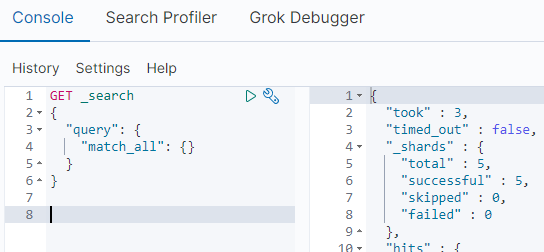
\includegraphics[scale=1.10]{images/kibanaConsole.PNG}
\end{figure}
Ein weiteres nützliches Feature ist die Möglichkeit sich die vergangenen Kommandos mithilfe des „History“ Reiters anzusehen und erneut auszuführen. Sehr praktisch ist auch die Autocomplete Funktion der Konsole, mit der man sich nicht nur einiges an Schreibaufwand spart, sondern auch bei der Fehlervermeidung hilft. Des Weiteren gibt es auch gut zehn verschiedene Shortcuts, mit denen man zum Beispiel die Dokumentation zu der derzeitigen Abfrage sich anzeigen lassen kann.
Natürlich kann auch über einen normalen REST Request auf die Datenbank zugegriffen werden, aber ich habe um Testdaten in den Prototypen zu bekommen diese Konsole verwendet, weil es für schnelle Daten Importe die einfachste Möglichkeit ist und außerdem die Syntax kontrolliert.
\subsection{REST Abfragen in der Konsole}
Es existieren natürlich auch hier die vier REST abfragen: 
\begin{itemize}
    \item GET (Nimmt Datensätze aus der DB)
    \item PUT (Updated bereits existierende Datensätze)
    \item POST (Erstellt neue Datensätze)
    \item DELETE (Löscht Datensätze)
\end{itemize}
Mit dem Kommando 
\begin{lstlisting}
PUT /indexname[/collectionname]
\end{lstlisting}
kann ein Index und bei Bedarf auch eine zugehörige Collection erstellt werden.
\subsection{Beispieldaten anlegen}
Nachdem wir nicht direkt auf die MIC-Datenbank zugreifen dürfen. Wurden mir einige Beispieldatensätze gegeben, um die Diagramme zu testen. Jedoch konnten die aus Oracle exportierten Datensätze nicht einfach in ES importiert werden, denn bei einigen Komma Werten wurde ein Beistrich anstatt eines Punktes gesetzt. Außerdem wurde das Oracle Datum nicht richtig erkannt, wodurch diese Felder extra bearbeitet werden mussten. 
Mit diesem Kommando können nun mehrere Datensätze importiert werden:
\begin{figure}[H]
    \centering
    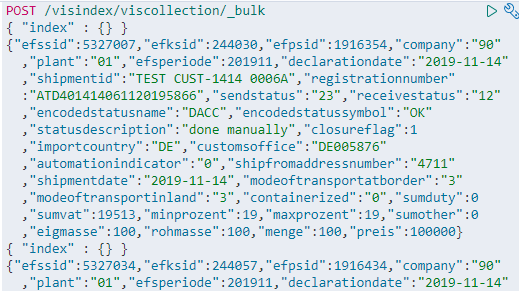
\includegraphics[scale=1.20]{images/kibanaConsole_dataImport.PNG}
\end{figure}
Um den Index mitsamt allen Daten nutzen zu können, muss nun ein „Index Pattern“ erstellt werden.
Dazu geht man unter den Einstellungen auf „Index Pattern“ und dort gibt man den Namen des bereits erstellten Index an. Es können auch Wildcards verwendet werden, um mehrere Indizes in ein „Index Pattern“ zu speichern. Im nächsten Schritt kann man noch einen Zeit Filter angeben. Dieser ist dazu da später in den Visualisierungen nach einer bestimmten Zeit zu filtern. Dieses Feature ist jedoch nur verfügbar, wenn die Datenbank ein Datumsfeld erkennt. 
Ist der Index nun erstellt, werden alle Felder angezeigt und gekennzeichnet, ob das jeweilige Feld suchbar und Aggregierbar ist. 
\section{Die Erstellung von Grafiken mit Kibana}
Über den Reiter „Visualize“ können die Bestehenden Visualisierungen angesehen und geändert werden und außerdem neue Erzeugt werden.
\begin{figure}[H]
    \centering
    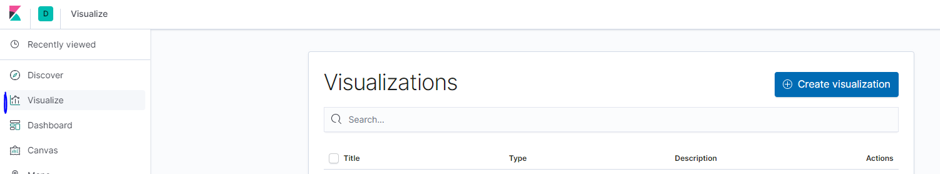
\includegraphics{images/vis_find.png}
\end{figure}
\subsection{Pie Chart}
Ein einfaches Pie Chart kann erstellt werden indem man auf den Button „Create Visualization“ klickt dann auf „Pie“ und anschließend die Datenquelle auswählt. Damit das Diagramm Werte bekommt, drückt man unter „Buckets“ „Add“ und wählt „Split splices“ aus. Als Aggregation kann man beliebig wählen aber mit „Terms“ können beliebige Felder aus der DB ausgewählt und aggregiert werden. Zum Schluss muss man sich nur noch ein Feld aussuchen und auf den blauen Button zu drücken. Ich habe nach dem Term: „encodedstatusname.keyword“ aggregiert. Somit kann man sich nun die Status aller Waren ansehen die gerade importiert werden. Falls keine Daten angezeigt werden ist wahrscheinlich das gesetzte Datum von dem die Daten genommen werden falsch.
\begin{figure}[H]
    \centering
    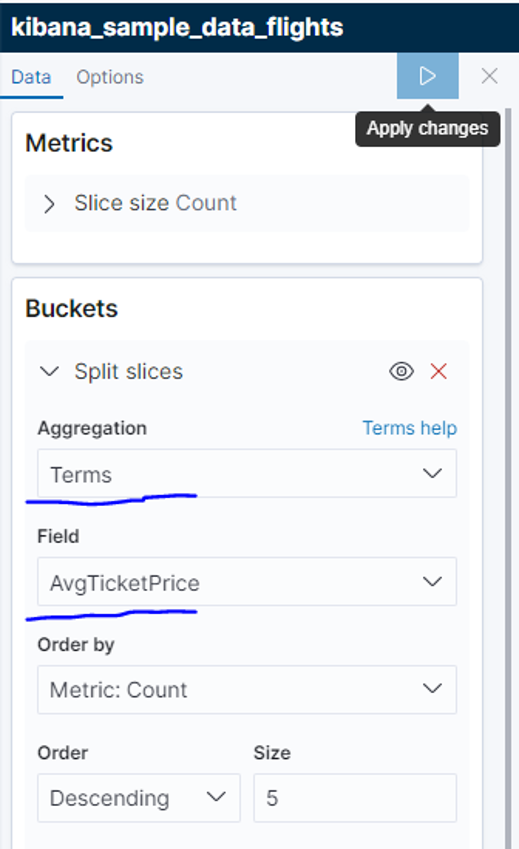
\includegraphics{images/vis_piechart.png}
\end{figure}
\subsection{Area Chart}
Um ein Area Chart zu erzeugen muss man einfach bei der Auswahl des Diagrammtyps „Area Chart“ auswählen und diesmal auch die Y-Achse bearbeiten
\begin{figure}[H]
    \subfigure[Y-Achse]{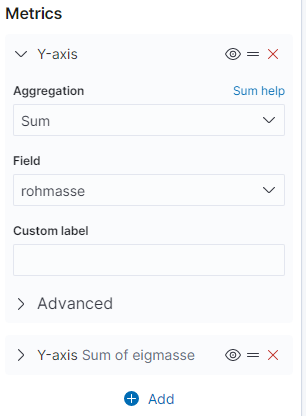
\includegraphics[width=0.49\textwidth]{images/kibanaChart_AreaLeft.PNG}}
    \subfigure[X-Achse]{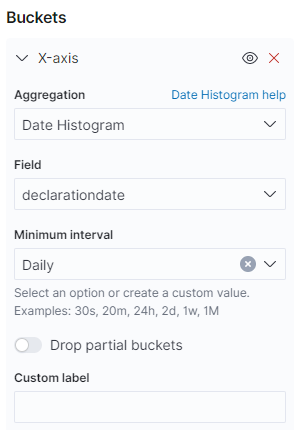
\includegraphics[width=0.49\textwidth]{images/kibanaChart_AreaRight.PNG}}
\caption{Area Chart Einstellungen}
\end{figure}
\subsection{Andere Diagrammarten}
Die wichtigsten Charts in Kibana haben alle denselben Aufbau wie das Area Chart. Es gibt noch viele Diagramme mehr doch Visualisierungen wie „Maps“ brauchen sehr spezifische Daten welche mit denen die wir zur Verfügung gestellt bekommen haben leider nicht enthalten. Grundsätzlich sind Maps etwas sehr Wertvolles für International agierende Unternehmen welche sehen wollen wie zum Beispiel die Verkaufszahlen pro Land aussehen oder unterschiedlich der Gewinn pro US Bundesstaat ist. 
\begin{figure}[H]
    \centering
    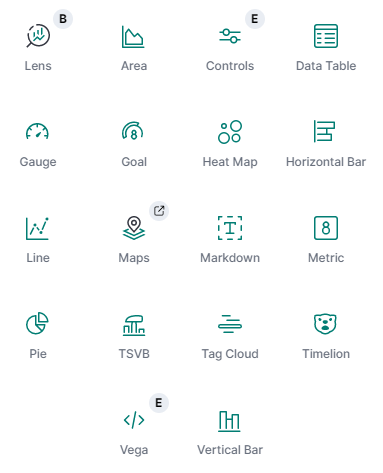
\includegraphics{images/kibanaChartAuswahl.PNG}
    \caption{Die große Auswahl an Diagrammarten}
\end{figure}
\section{Das Dashboard}
Dashboards sind eine tolle Möglichkeit verschiedenste Diagramme auf einen Blick zugänglich zu machen. In Kibana geht das erstellen von Dashboards so einfach wie Möglich denn man kann die zuvor erstellten Diagramme mit zweit Klicks hinzufügen und so Positionieren wie man es braucht. Die Diagramme skalieren dabei bei Größen Änderungen aktiv mit. Hervorragend ist außerdem die Interaktivität der Diagramme im Dashboard denn man kann mit einem Klick in einem Diagramm das ganze Dashboard auf zum Beispiel ein Produkt abzielen lassen. Außerdem kann man die Zeitspanne aus der die Daten angezeigt werden verändern indem man den gewünschten Bereich in einem der Diagramme mit der Maus markiert. Nach der Markierung ändern sich Zeitintervalle der anderen Diagramme ebenso.
\begin{figure}[H] 
    \centering
    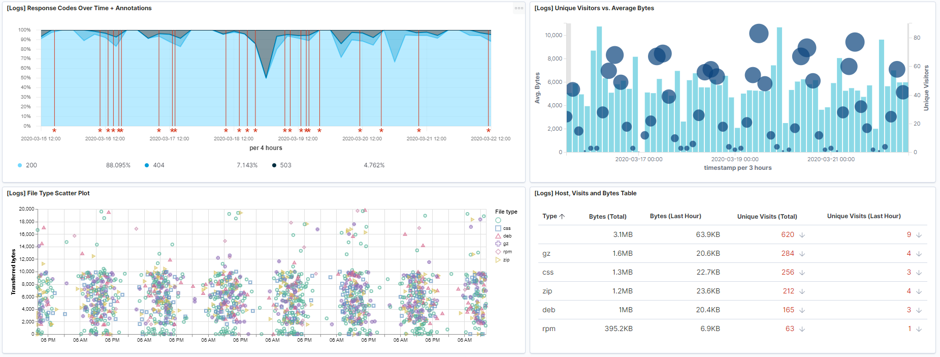
\includegraphics[scale=0.9]{images/dashboard.png}
    \caption{Ein Beispiel für ein Dashboard}
\end{figure}
\section{Probleme beim Visualisierungsprozess}
\subsection{AWS und das MIC Firmennetzwerk}
Bei MIC gab es keinen der wirklich mit AWS umzugehen wusste und wir waren somit die Testobjekte denn diese Diplomarbeit hätte genauso gut auf einem beliebigen Server oder Desktop PC laufen können. Als erstes habe ich probiert über den Standard Port 5601 auf Kibana zuzugreifen was jedoch nicht funktionierte, weil das Firmennetzwerk von MIC lässt PCs darin nur auf Port 80 (http) zugreifen. Ich habe also nun versucht den Docker Container so umzuschreiben damit Port 80 verwendet wird jedoch wollte die VM das nicht zulassen. Der nächste Versuch bestand darin einen Nginx [\ref{sec:nginx}] Server aufzusetzen welcher die Kibana User-Interface auf Port 80 weiterleitet. Davon abzusehen, dass es ewig dauerte bis der aufgesetzt war, weil die Konfiguration nicht stimmte leitete er ordnungsgemäß auf Port 80 weiter. Das letzte Problem bestand nun darin die AWS VM zu überzeugen das Port 80 offen sein soll. Dazu musste ich eine „Security Group“ erstellen in welcher dann die „Inbound und Outbound Rules“ festgelegt werden konnten. 
\subsection{Der Datenimport}
Das Hauptproblem beim Datenimport war das in der Dokumentation der REST API der Datenimport von vielen Datensätzen in einer Anfrage nicht beschrieben wurde. Ich musste daraufhin über die „Bulk“ API ausweichen. Des Weiteren musste der Oracle Output der Beispieldaten umgeformt werden denn die Punkte bei Kommazahlen wurden als Beistrich in das Ausgabefile geschrieben und die REST API erkannte die Datumsformatierung nicht sodass ich jedes Datum umformen musste.
